\subsection{Checkout - Customer Info}

%For the main pages put a mockup and describe it in detail.

%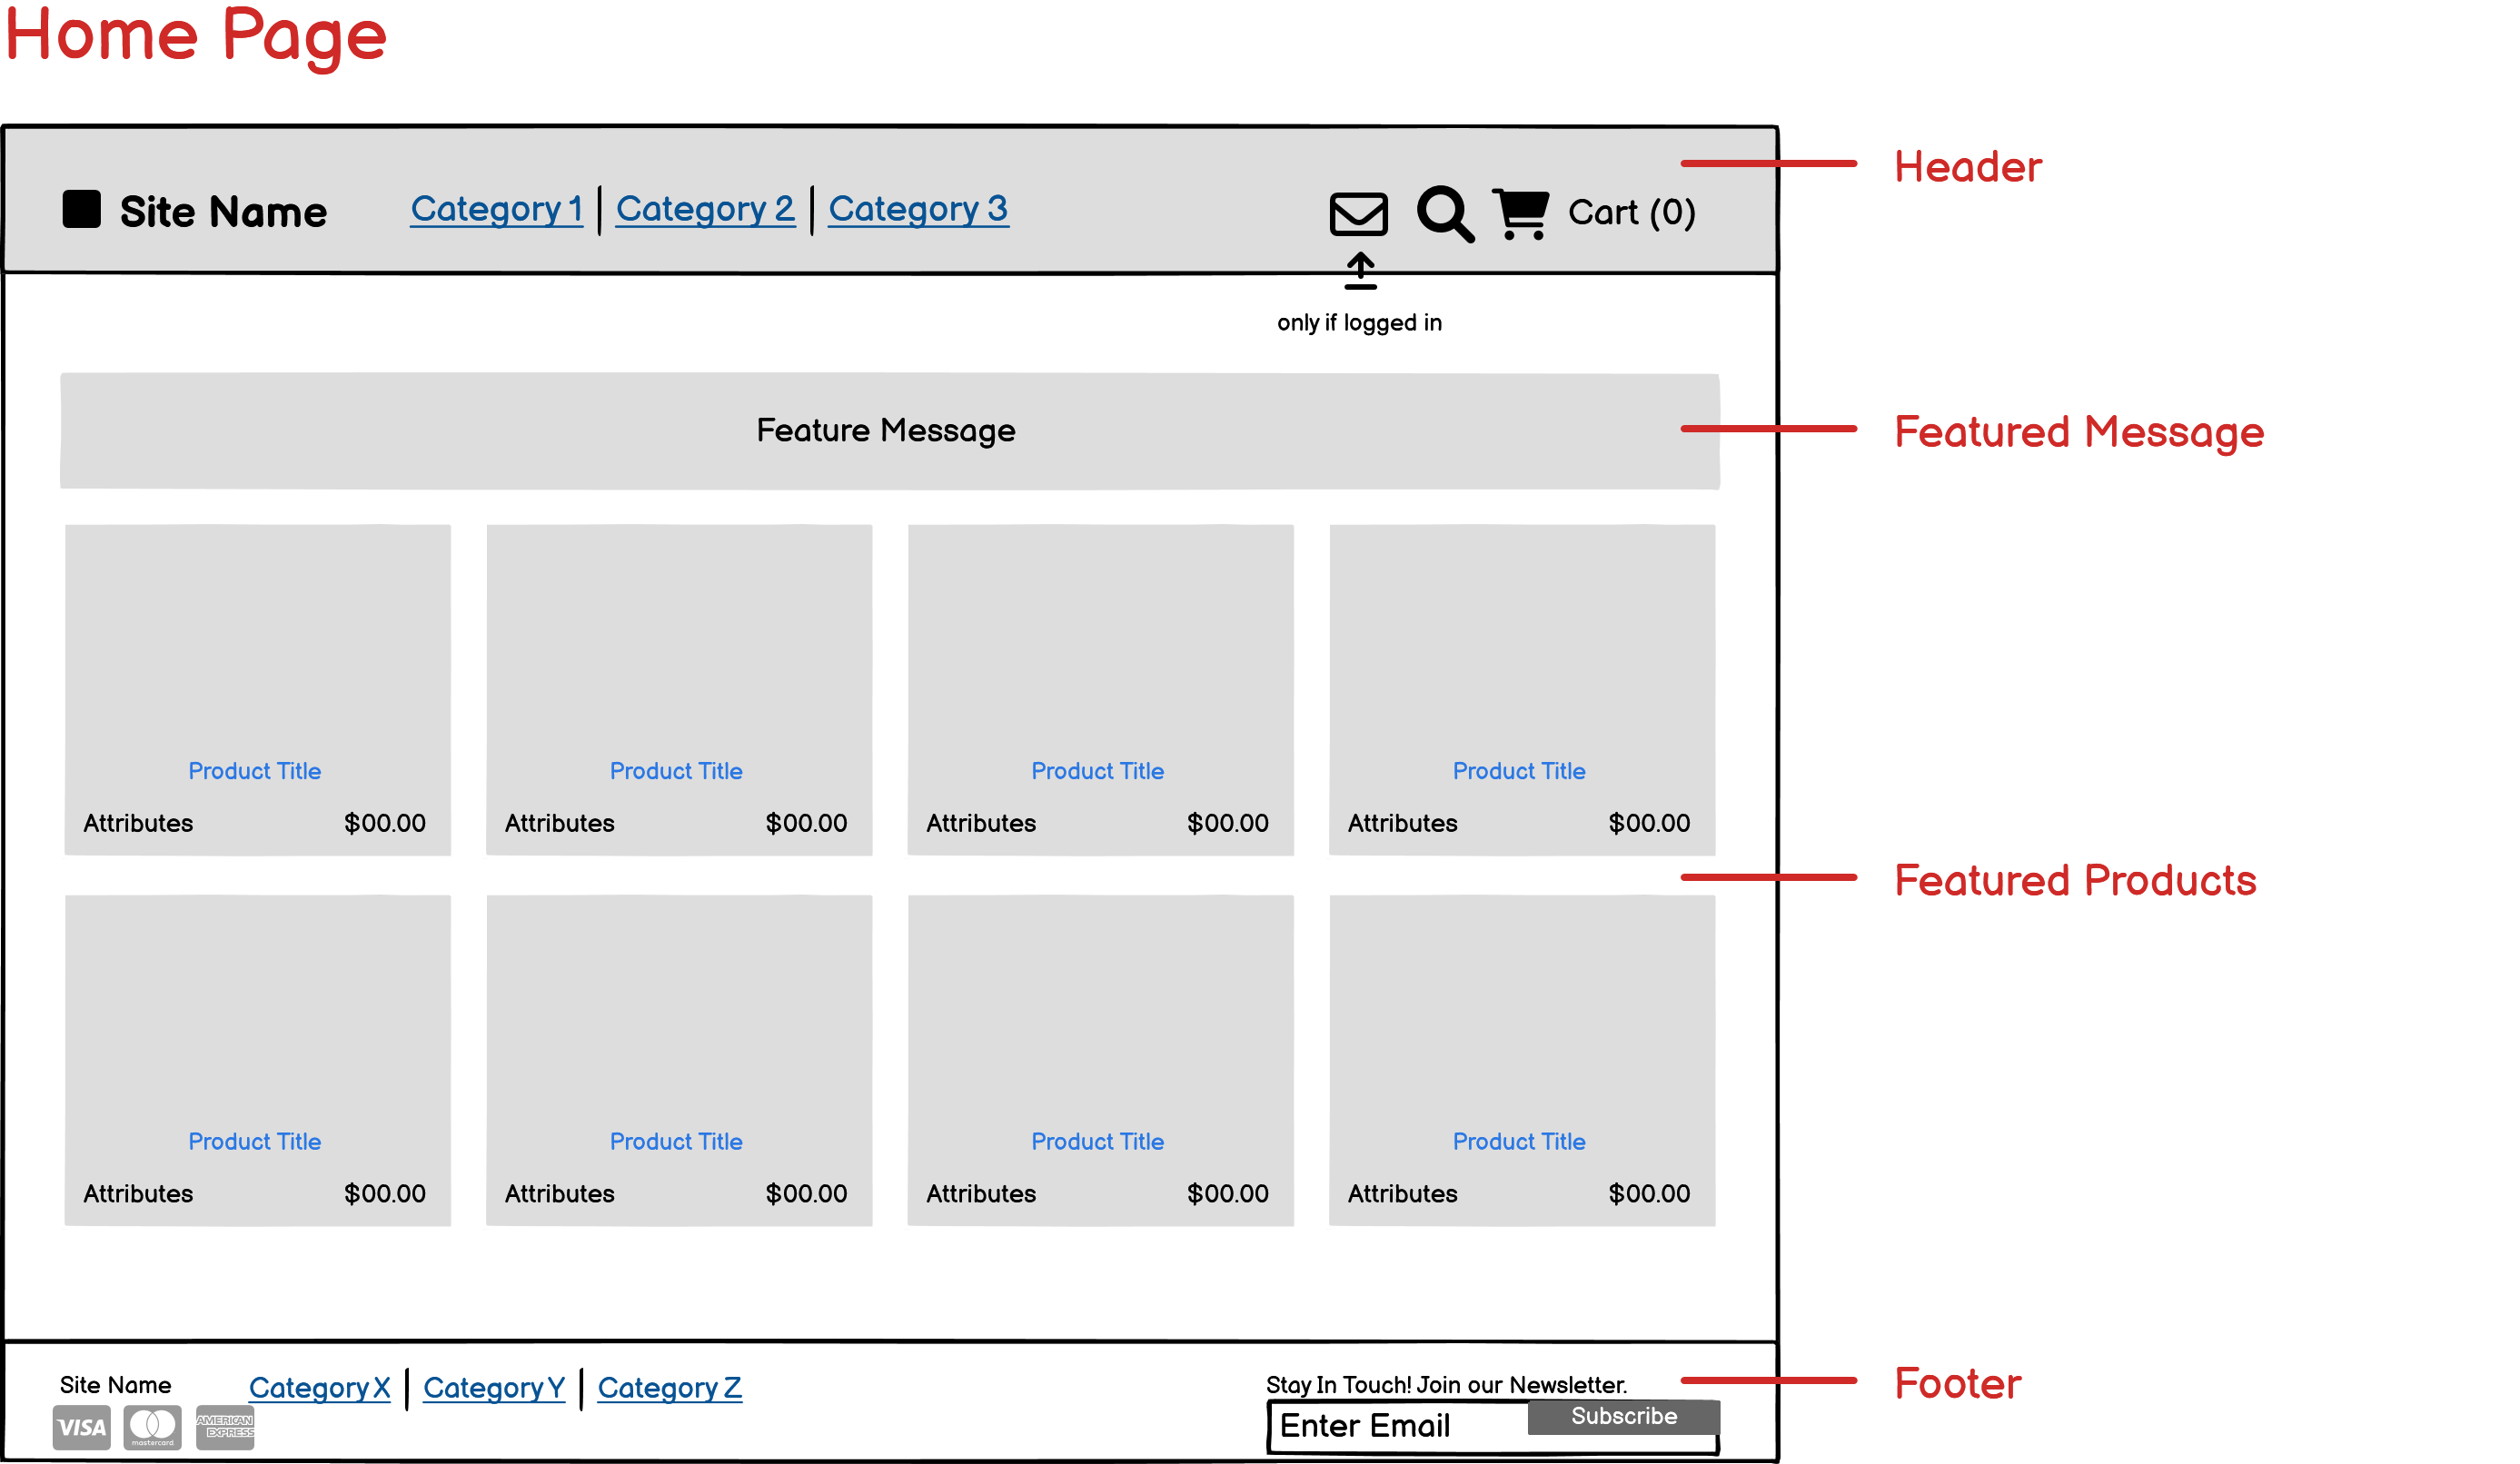
\includegraphics[scale=0.5]{logos/Images/pages/Home Page.png}

\begin{figure}[h]
    \centering
    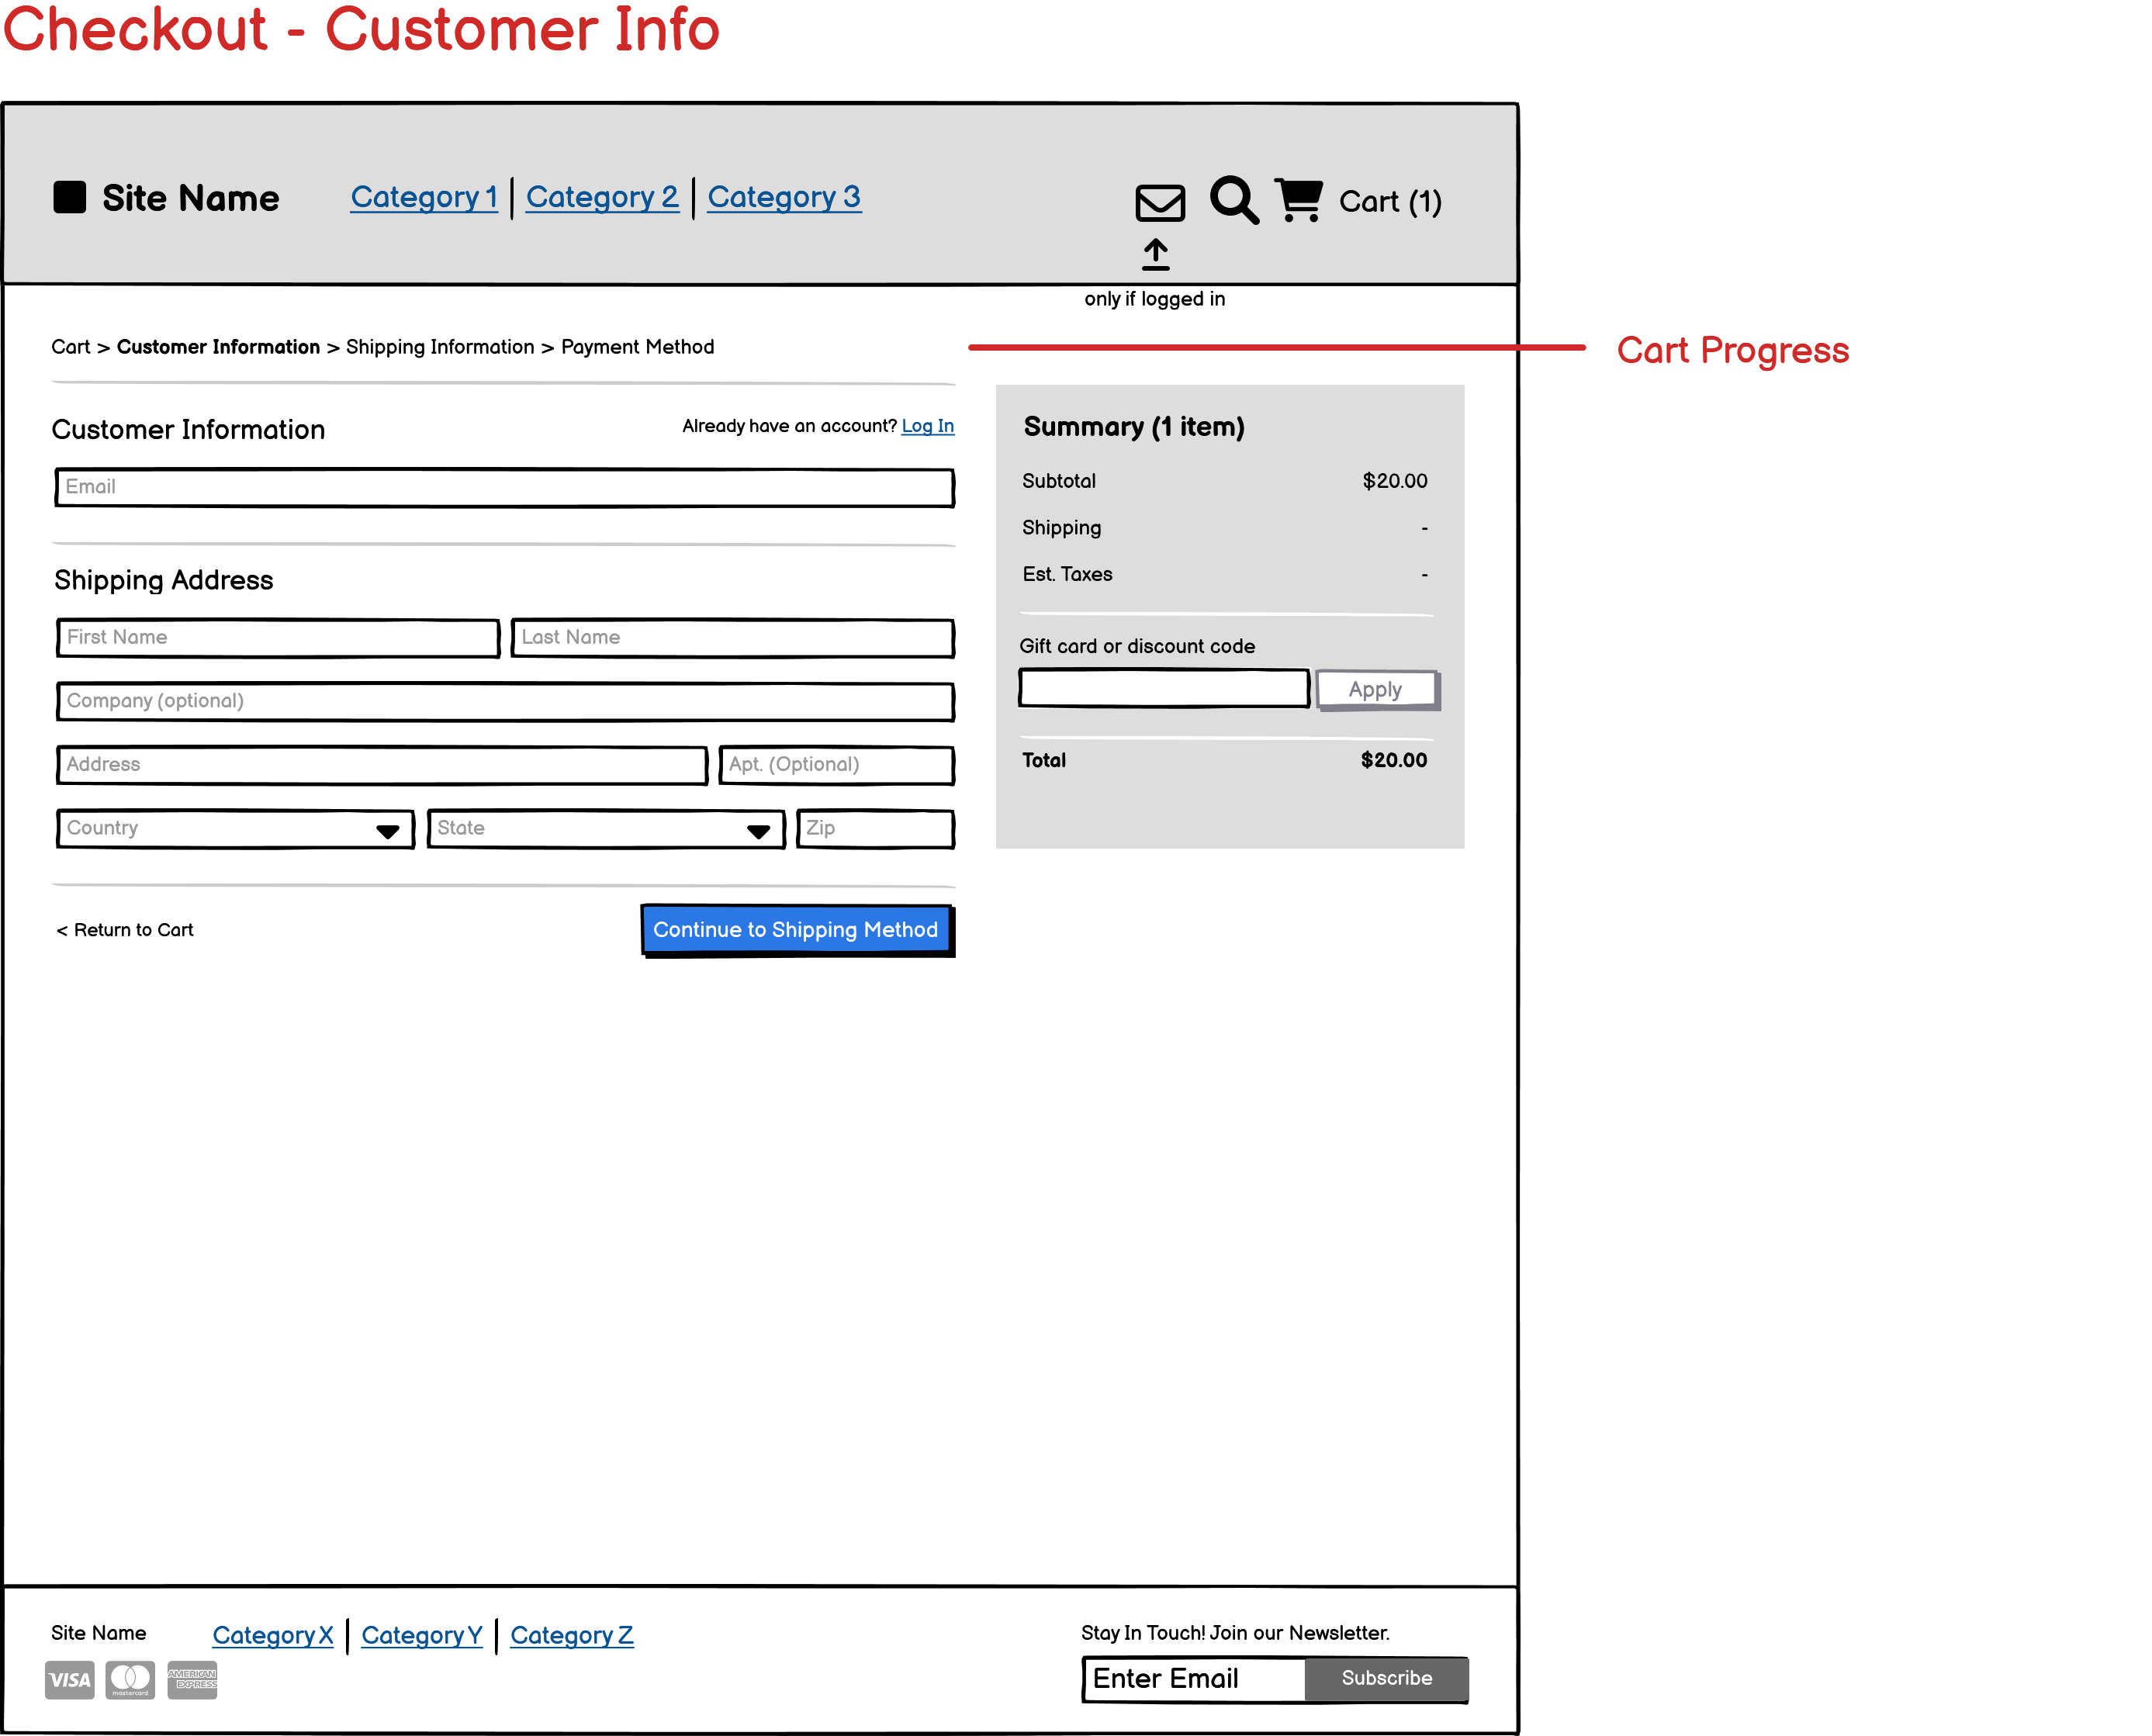
\includegraphics[scale=0.5]{logos/Images/pages/Checkout - Customer Info.png}
    \caption{Checkout - Customer Info}
    \label{fig:my_label}
\end{figure}
\hfill \break
On the customer information page, the user is shown various fields where he can enter his personal information. This includes first name, last name, company name, address, country, city and zip code.\\\\
The purpose of this page is to ensure that the order is sent to the correct address. The user must enter the exact address here in order for the delivery to be completed successfully.\\\\
In addition to this, the user can also log in with their account on this page if they already have one. This can speed up the ordering process, as the user does not have to enter all personal data again.\\\\
The customer information page is an important step in the ordering process, as it ensures that the order is sent to the correct address and keeps the user updated. It is important that the user enters accurate and up-to-date information to ensure that the order is completed successfully.